\section{Examples}

	\subsection{Example 1 - polynomial}
		\subsubsection{Equation}
		The equation solved is
		\begin{equation}
			-\Delta u = f
		\end{equation}

		in the domain $\Omega = (0, 4)^2$, equipped with a Dirichlet
		boundary conditions given by the exact solution.

		\subsubsection{Exact solution}
		The exact solution reads
		\begin{equation}
			u(x, y) = f(x) f(y), f(a) = a\left(a-1\right)\left(a-2\right)\left(a-3\right)\left(a-4\right).
		\end{equation}
		\begin{figure}[H]
			\centering
			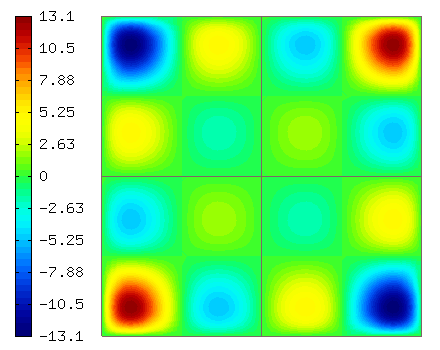
\includegraphics[height=5cm]{img/exact-polynom.png}
			\caption{Exact solution}
			\label{fig:exact-polynom}
		\end{figure}

		TODO: probrat co se ma ukazat (viz mail)



	\newpage
	\subsection{Example 2 - trigonometric}
		\subsubsection{Equation}
		The equation solved is
		\begin{equation}
			-\Delta u = f
		\end{equation}

		in the domain $\Omega = (0, \pi)^2$, equipped with a Dirichlet
		boundary conditions given by the exact solution.

		\subsubsection{Exact solution}
		The exact solution reads
		\begin{equation}
			u(x, y) = f(x) f(y), f(a) = sin(a).
		\end{equation}
		\begin{figure}[H]
			\centering
			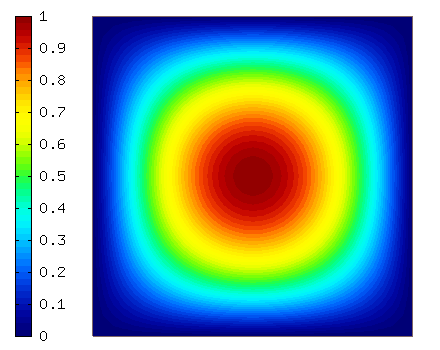
\includegraphics[height=5cm]{img/exact-sin.png}
			\caption{Exact solution}
			\label{fig:exact-sin}
		\end{figure}

		\subsubsection{Problem for adaptivity algorithms}
			The problem arises in the use of p-adaptivity. Starting from an initial mesh consisting of only one element of the 2-nd order, the reference space consists also of one element of the 3-rd order. These two FE spaces yield the same solution:
			\begin{figure}[H]
				\centering
				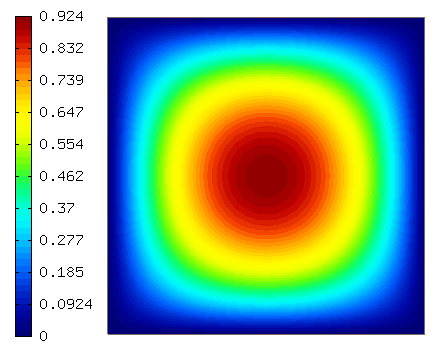
\includegraphics[height=5cm]{img/sin-p.png}
				\caption{p-adaptivity solution}
				\label{fig:exact-sin}
			\end{figure}
			
			For all the following convergence plots, the prescribed relative error in $H^1$ norm was $1e-8\%$. It was not reached by the 2nd-order h-adaptive scheme.
		
		\subsubsection{Convergence plots - h-adaptivity, 2-nd degree elements}
			\begin{figure}[H]
				\centering
				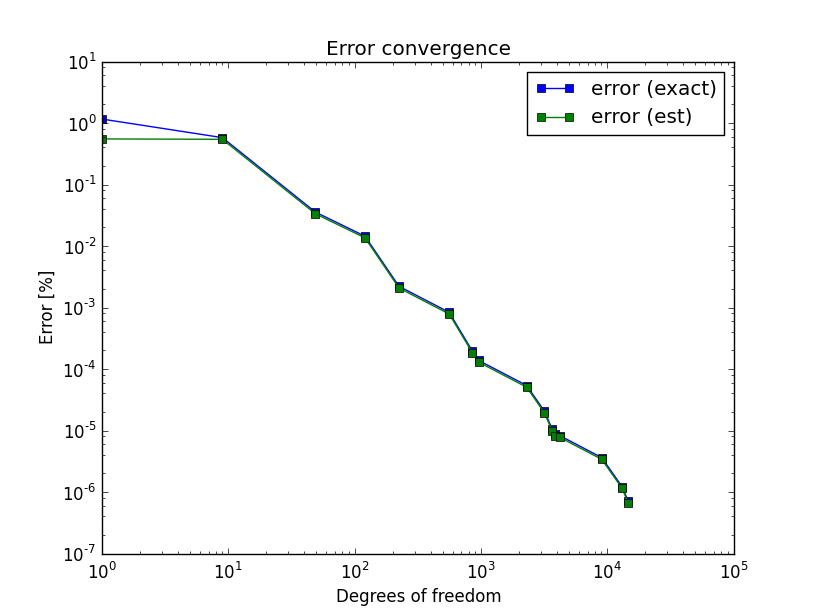
\includegraphics[height=5cm]{img/sin-h2-dof.png}
				\caption{Relative (H1) error wrt. degrees of freedom}
			\end{figure}
			
			\begin{figure}[H]
				\centering
				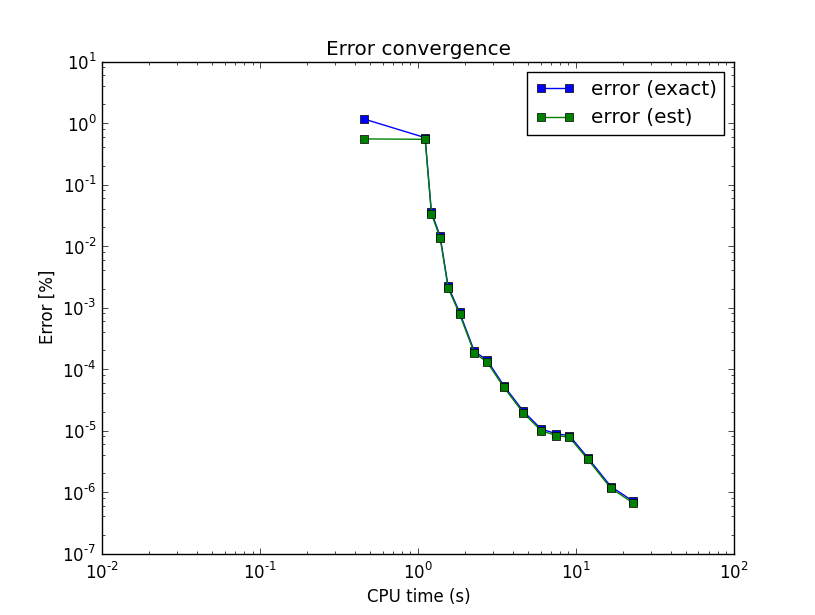
\includegraphics[height=5cm]{img/sin-h2-cpu.png}
				\caption{Relative (H1) error wrt. CPU time}
			\end{figure}
			
		\subsubsection{Convergence plots - h-adaptivity, 3-nd degree elements}
			\begin{figure}[H]
				\centering
				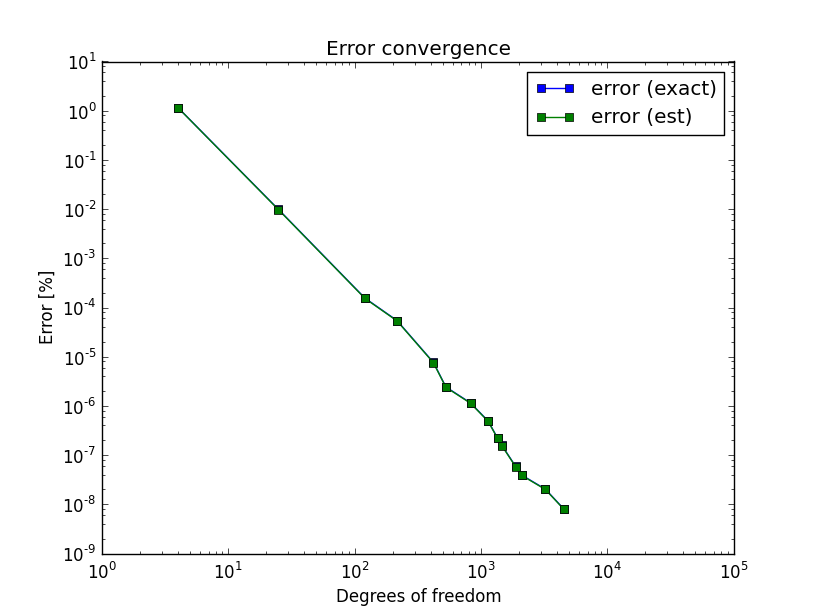
\includegraphics[height=5cm]{img/sin-h3-dof.png}
				\caption{Relative (H1) error wrt. degrees of freedom}
			\end{figure}
			
			\begin{figure}[H]
				\centering
				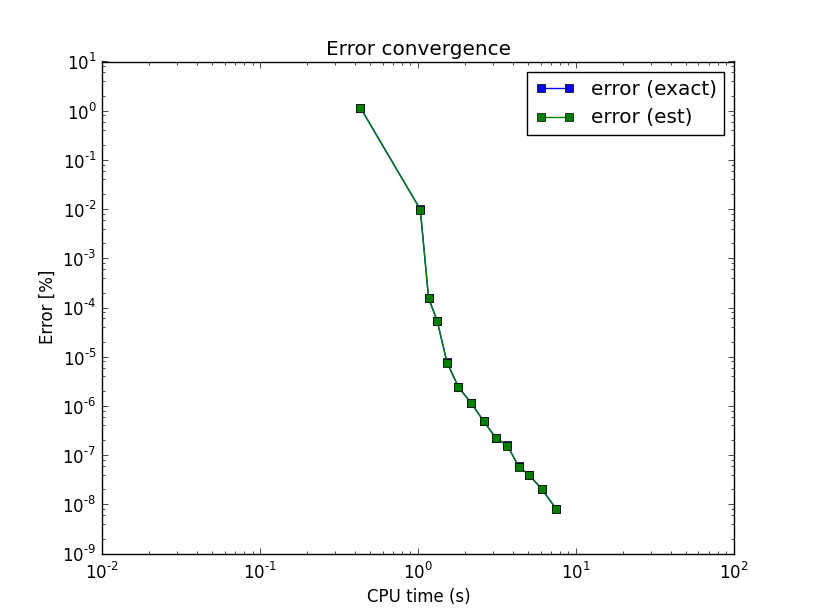
\includegraphics[height=5cm]{img/sin-h3-cpu.png}
				\caption{Relative (H1) error wrt. CPU time}
			\end{figure}
			
		\subsubsection{Convergence plots - hp-adaptivity}
			\begin{figure}[H]
				\centering
				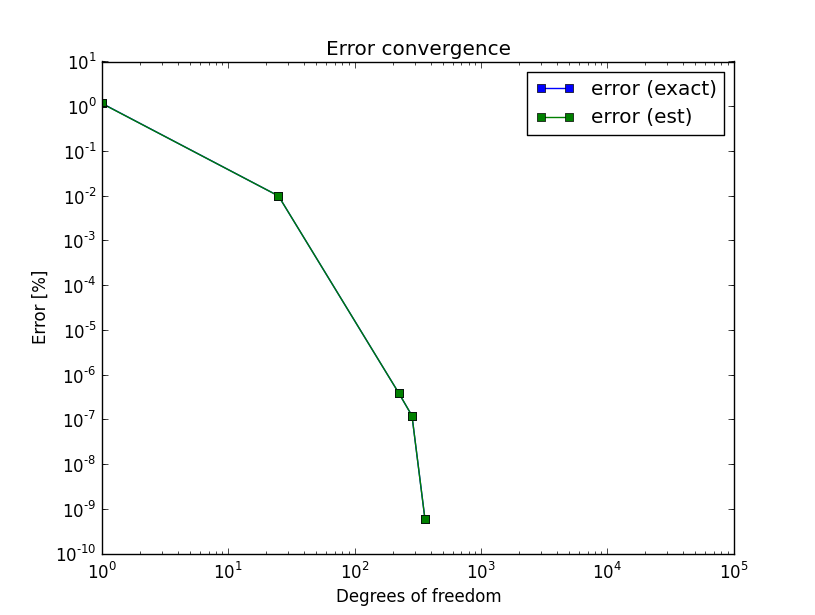
\includegraphics[height=5cm]{img/sin-hp-dof.png}
				\caption{Relative (H1) error wrt. degrees of freedom}
			\end{figure}
			
			\begin{figure}[H]
				\centering
				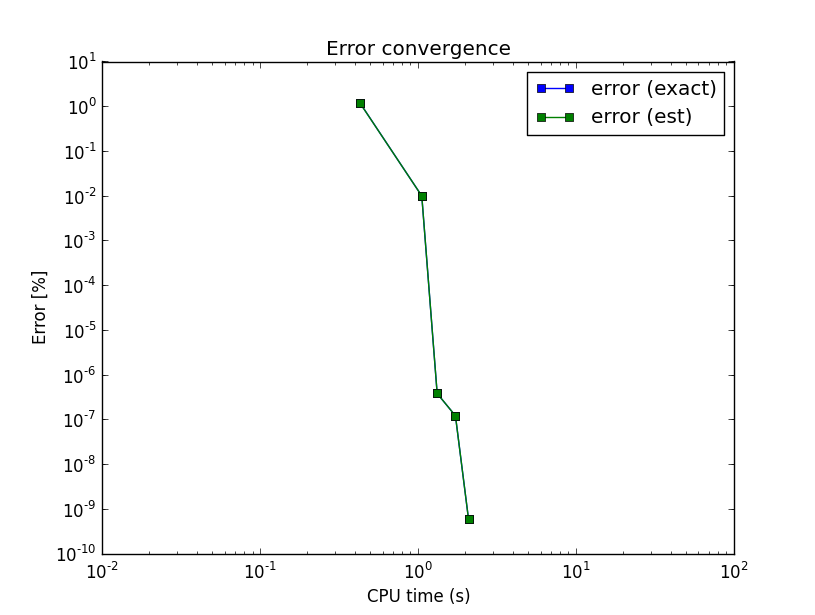
\includegraphics[height=5cm]{img/sin-hp-cpu.png}
				\caption{Relative (H1) error wrt. CPU time}
			\end{figure}



	\newpage
	\subsection{Example 3 - trigonometric high frequency}
		\subsubsection{Equation}
		The equation solved is
		\begin{equation}
			-\Delta u = f
		\end{equation}

		in the domain $\Omega = (0, \pi)^2$, equipped with a Dirichlet
		boundary conditions given by the exact solution.

		\subsubsection{Exact solution}
		The exact solution reads
		\begin{equation}
			u(x, y) = f(x) f(y), f(a) = sin(100*a).
		\end{equation}
		\begin{figure}[H]
			\centering
			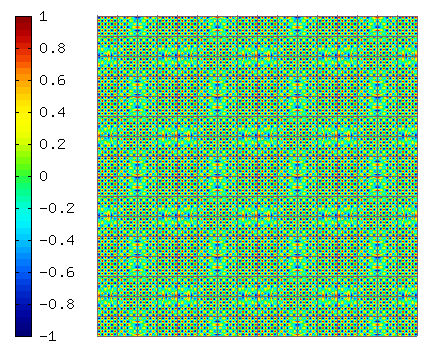
\includegraphics[height=5cm]{img/exact-sin100.png}
			\caption{Exact solution}
			\label{fig:exact-sin100}
		\end{figure}

		\subsubsection{Problem for adaptivity algorithms}
		
			
			For all the following convergence plots, the prescribed relative error in $H^1$ norm was $1e-1\%$. It was not reached by any scheme.
		
		\subsubsection{Convergence plots - h-adaptivity, 2-nd degree elements}
			\begin{figure}[H]
				\centering
				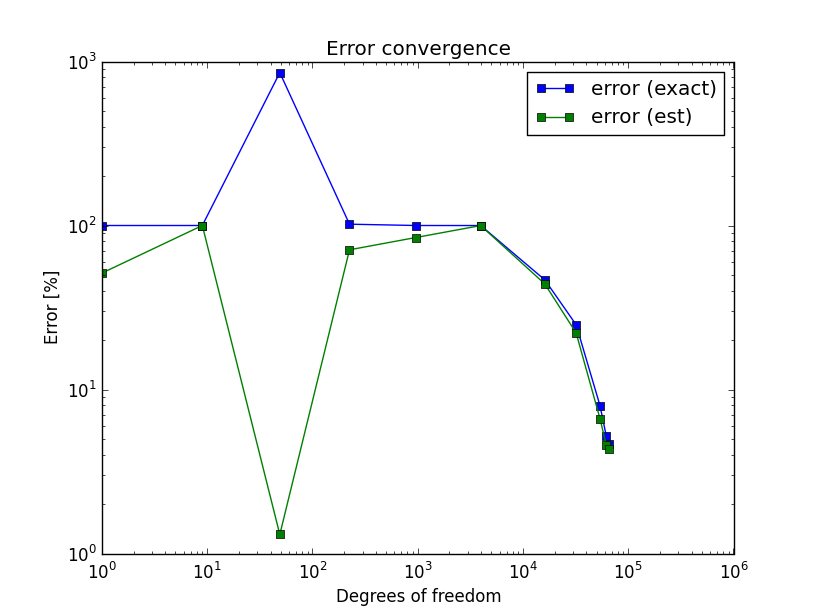
\includegraphics[height=5cm]{img/sin100-h2-dof.png}
				\caption{Relative (H1) error wrt. degrees of freedom}
			\end{figure}
			
			\begin{figure}[H]
				\centering
				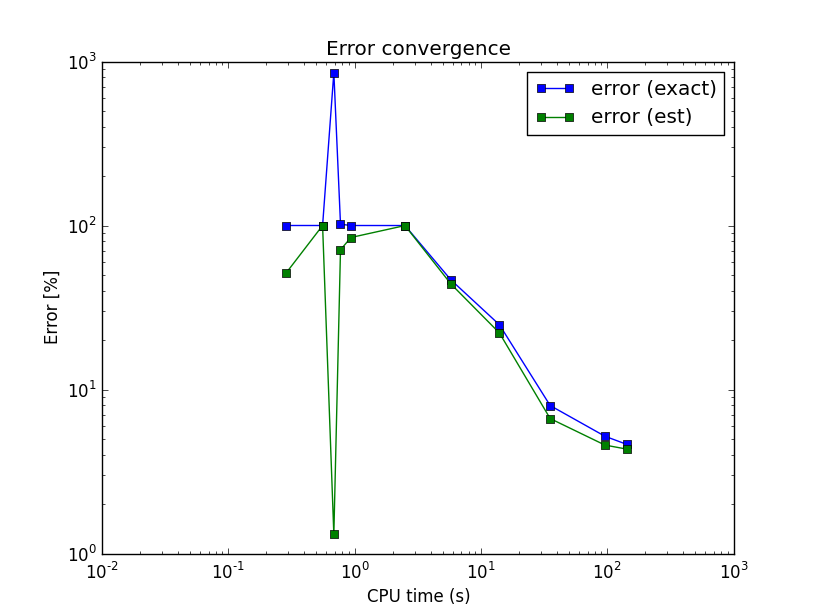
\includegraphics[height=5cm]{img/sin100-h2-cpu.png}
				\caption{Relative (H1) error wrt. CPU time}
			\end{figure}
			
		\subsubsection{Convergence plots - h-adaptivity, 3-nd degree elements}
			\begin{figure}[H]
				\centering
				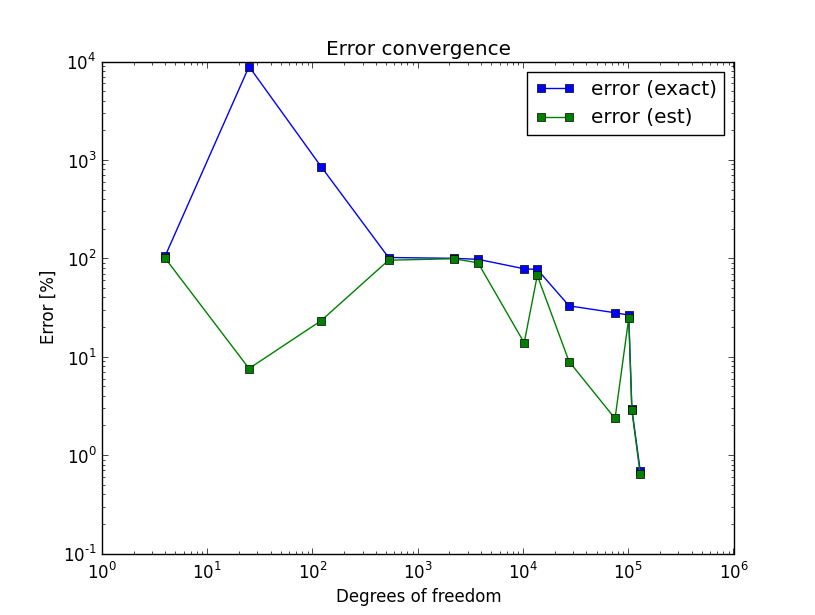
\includegraphics[height=5cm]{img/sin100-h3-dof.png}
				\caption{Relative (H1) error wrt. degrees of freedom}
			\end{figure}
			
			\begin{figure}[H]
				\centering
				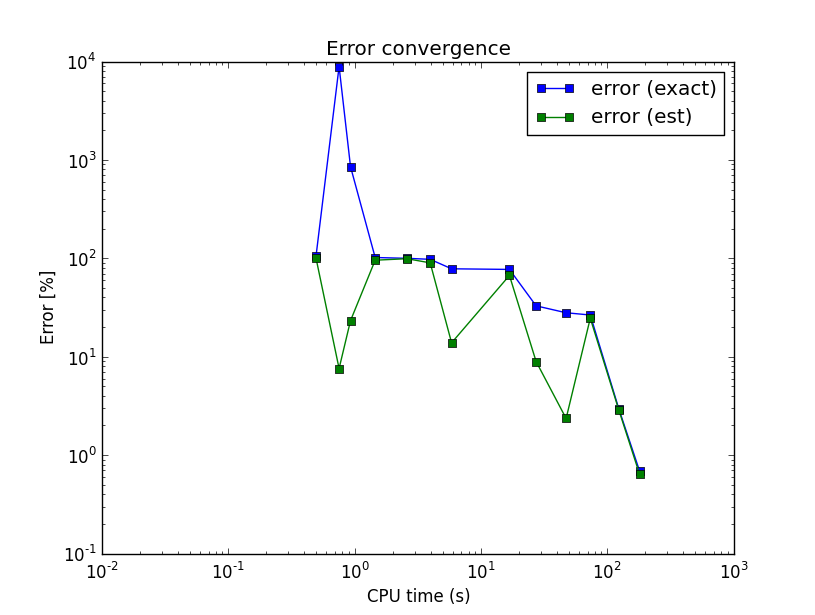
\includegraphics[height=5cm]{img/sin100-h3-cpu.png}
				\caption{Relative (H1) error wrt. CPU time}
			\end{figure}
			
		\subsubsection{Convergence plots - hp-adaptivity}
			\begin{figure}[H]
				\centering
				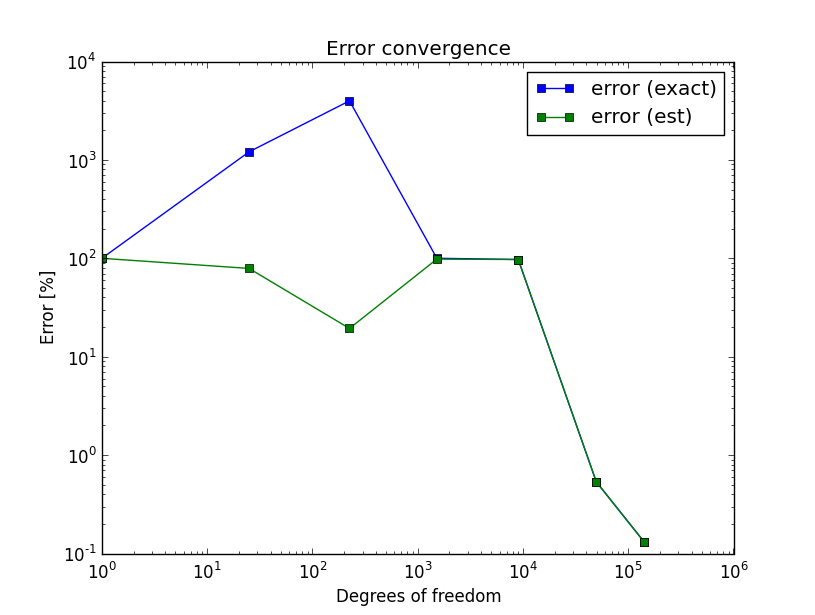
\includegraphics[height=5cm]{img/sin100-hp-dof.png}
				\caption{Relative (H1) error wrt. degrees of freedom}
			\end{figure}
			
			\begin{figure}[H]
				\centering
				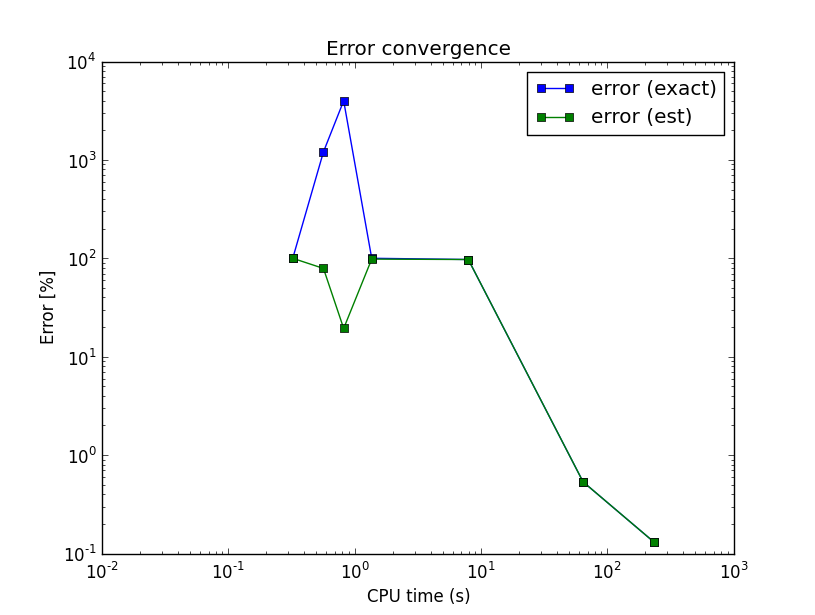
\includegraphics[height=5cm]{img/sin100-hp-cpu.png}
				\caption{Relative (H1) error wrt. CPU time}
			\end{figure}
			
			Final hp-mesh yielding $142032$ degrees of freedom and relative error of $~0.131\%$.
			\begin{figure}[H]
				\centering
				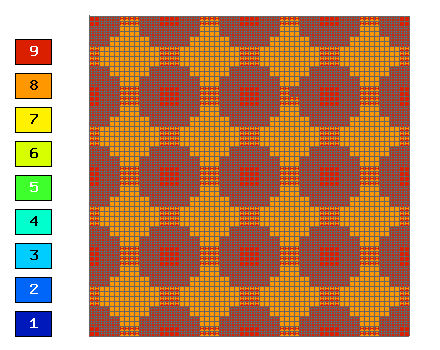
\includegraphics[height=5cm]{img/sin100-hp-finalmesh.png}
				\caption{Final hp-mesh}
			\end{figure}


	\newpage
	\subsection{Example 4 - intersecting interfaces}
		\subsubsection{Equation}
		The equation solved is
		\begin{equation}
			-\nabla \cdot (a(x,y) \nabla u) = 0,
		\end{equation}
		where the parameter $a$ is piecewise-constant,
		$a(x,y) = 161.4476387975881$ in the first and third quadrants,
		and $a(x,y) = 1$ in the remaining two quadrants.

		in the domain $\Omega = (-1, 1)^2$, equipped with a Dirichlet
		boundary conditions given by the exact solution.

		\subsubsection{Exact solution}
		The exact solution reads
		\begin{equation}
			u(x,y) = r^{a_1} \mu (\theta),
		\end{equation}
		where $a_1$ and $\mu (\theta)$ is given in \cite{mitchell-1}.
		\begin{figure}[H]
			\centering
			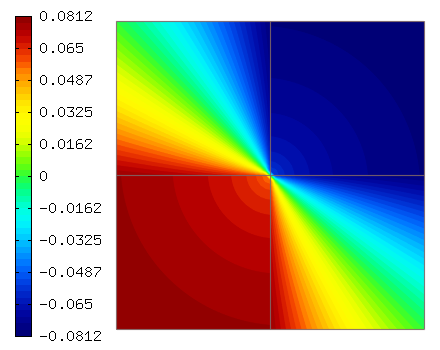
\includegraphics[height=5cm]{img/exact-kellog.png}
			\caption{Exact solution}
			\label{fig:exact-kellog}
		\end{figure}
		
		\subsubsection{Problem for adaptivity algorithms}
		
			For all the following convergence plots, the prescribed relative error in $H^1$ norm was $1e-3\%$. It was not reached by the 2nd-order h-adaptive scheme.
		
		\subsubsection{Convergence plots - h-adaptivity, 2-nd degree elements}
			\begin{figure}[H]
				\centering
				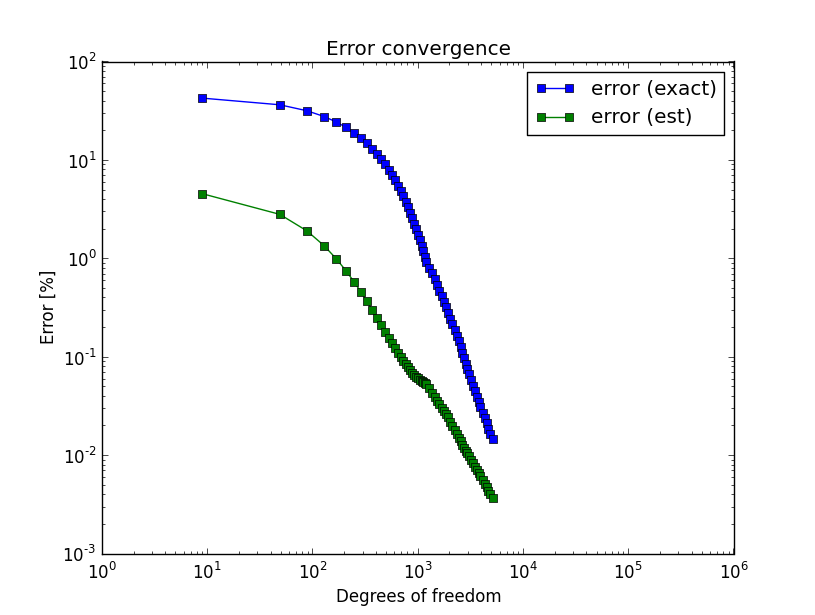
\includegraphics[height=5cm]{img/kellog-h2-dof.png}
				\caption{Relative (H1) error wrt. degrees of freedom}
			\end{figure}
			
			\begin{figure}[H]
				\centering
				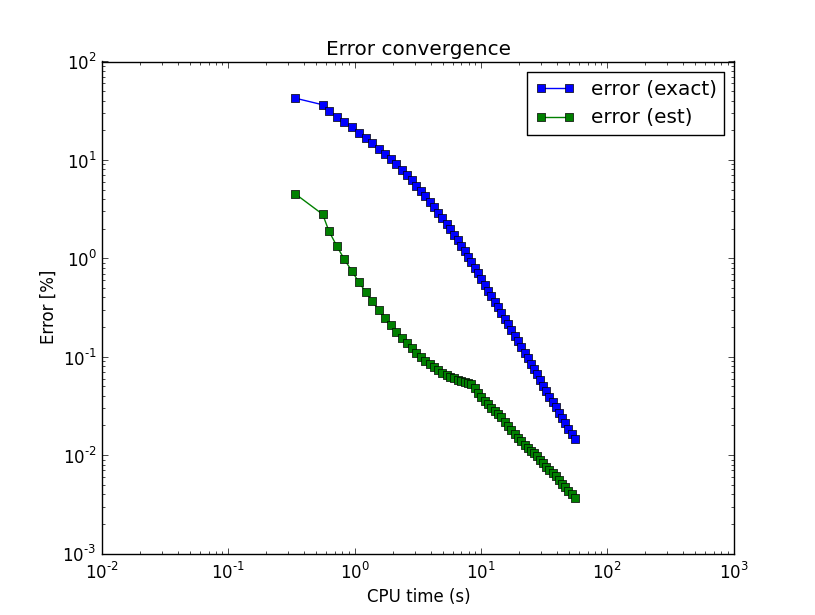
\includegraphics[height=5cm]{img/kellog-h2-cpu.png}
				\caption{Relative (H1) error wrt. CPU time}
			\end{figure}
			
			Final mesh yielding $5185$ degrees of freedom and relative error of $~0.0036\%$.
			\begin{figure}[H]
				\centering
				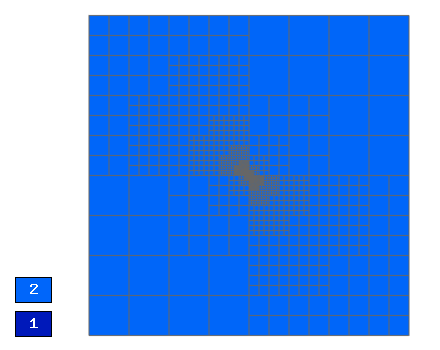
\includegraphics[height=5cm]{img/kellog-h2-finalmesh.png}
				\caption{Final mesh - 2nd order}
			\end{figure}
			
		\subsubsection{Convergence plots - h-adaptivity, 3-nd degree elements}
			\begin{figure}[H]
				\centering
				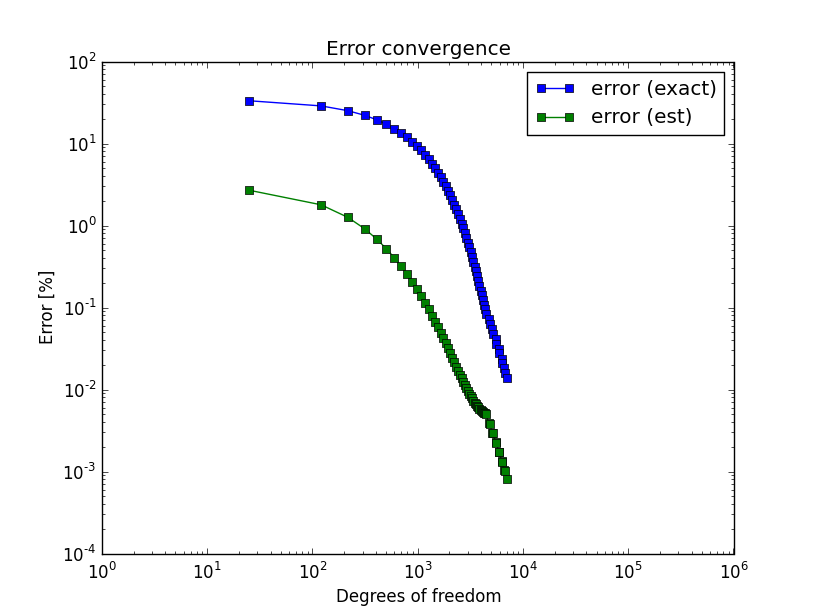
\includegraphics[height=5cm]{img/kellog-h3-dof.png}
				\caption{Relative (H1) error wrt. degrees of freedom}
			\end{figure}
			
			\begin{figure}[H]
				\centering
				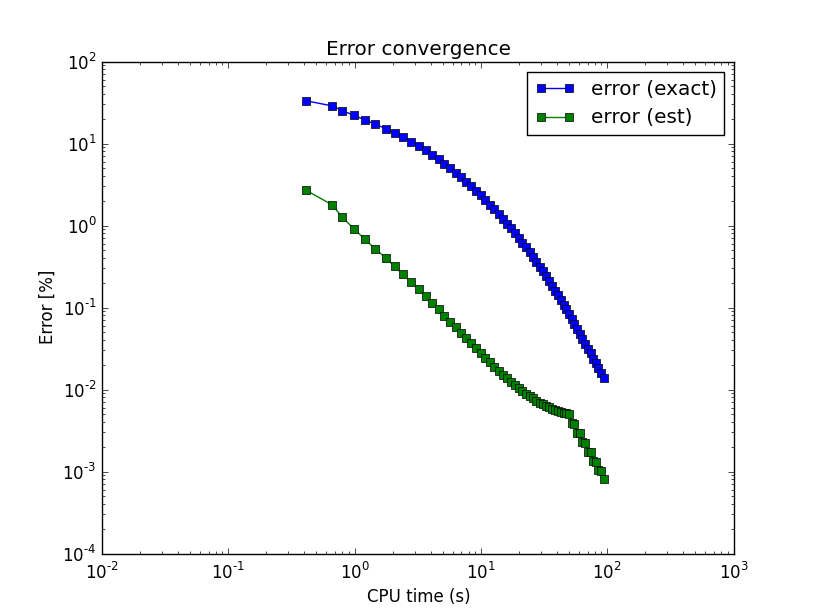
\includegraphics[height=5cm]{img/kellog-h3-cpu.png}
				\caption{Relative (H1) error wrt. CPU time}
			\end{figure}
			
			
			Final mesh yielding $7078$ degrees of freedom and relative error of $~0.00092\%$.
			\begin{figure}[H]
				\centering
				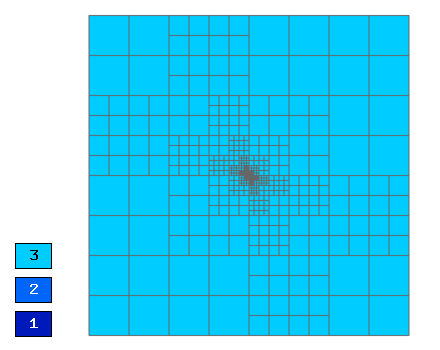
\includegraphics[height=5cm]{img/kellog-h3-finalmesh.png}
				\caption{Final mesh - 3rd order}
			\end{figure}
			
		\subsubsection{Convergence plots - hp-adaptivity}
			\begin{figure}[H]
				\centering
				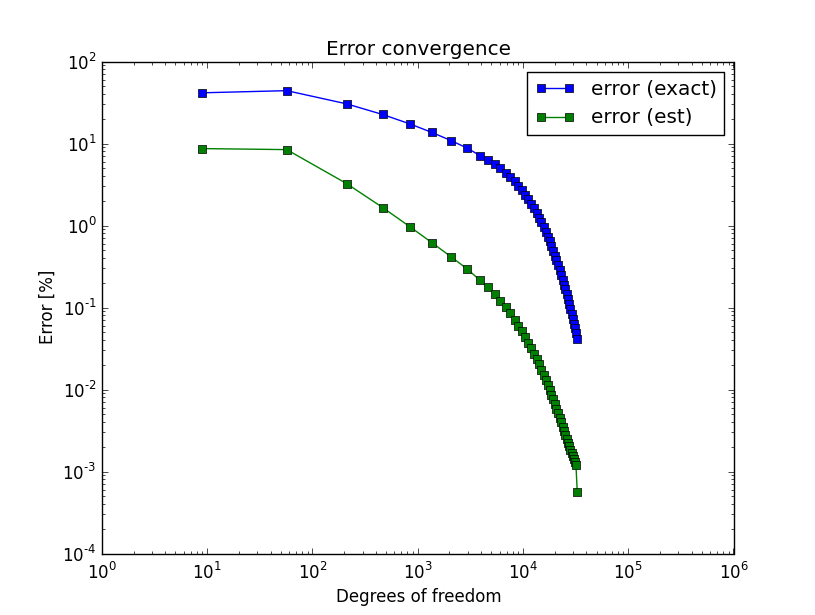
\includegraphics[height=5cm]{img/kellog-hp-dof.png}
				\caption{Relative (H1) error wrt. degrees of freedom}
			\end{figure}
			
			\begin{figure}[H]
				\centering
				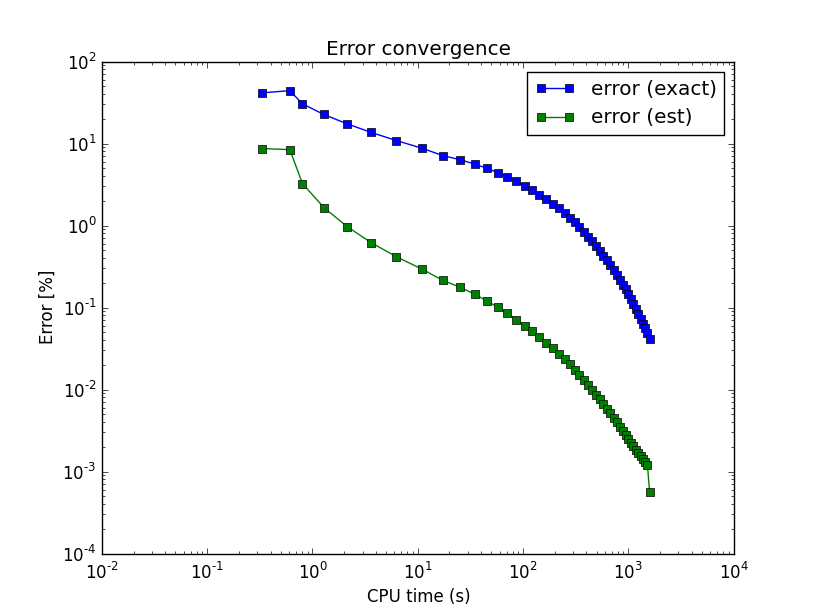
\includegraphics[height=5cm]{img/kellog-hp-cpu.png}
				\caption{Relative (H1) error wrt. CPU time}
			\end{figure}
			
			Final hp-mesh yielding $32801$ degrees of freedom and relative error of $~0.00056\%$.
			\begin{figure}[H]
				\centering
				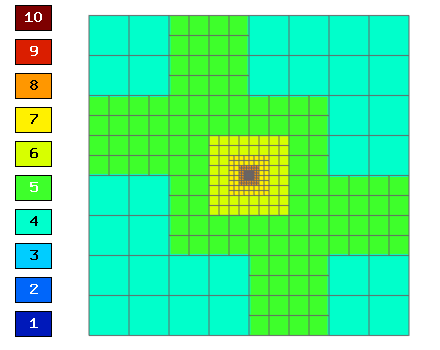
\includegraphics[height=5cm]{img/kellog-hp-finalmesh.png}
				\caption{Final hp-mesh}
			\end{figure}

\newpage
\subsection{Example 5 - acoustic wave}
\subsubsection{Equation}
	The equation solved is
	\begin{equation}
		-\ \mathrm{div} \left( \frac{1}{\rho}\,\, \nabla p \right) + \frac{1}{\rho  c^2} \frac{\partial^2 p}{\partial t^2} = 0,
	\end{equation}
	where $\rho$ is the acoustic density $\left(\rho = 1.25\right)$, and $c$ is the acoustic speed $\left(c = 1.25\right)$.\ \\
	We solve the equation	in the time interval $\left[0, \infty \right]$ in the domain $\Omega = (0, 4) * (0, 3)$, with the following boundary conditions:
	\begin{eqnarray}
	  \frac{\partial p}{\partial n} & = & 0,\ t \in \left[0, \infty \right]\ on\ \{4\} * \left[0, 3\right] \\
		p & = & \sin\left(2\pi f t\right),\ f = 800,\ t \in \left[0, 1 \right],\ on\ \{0\} * \left[0, 3\right] \\
		p & = & 0,\ t > 1,\ on\ \{0\} * \left[0, 3 \right] \\
		\frac{1}{\rho} \frac{\partial p}{\partial n} & = & - \frac{1}{c\rho} \frac{\partial p}{\partial t},\ t \in \left[0, \infty \right],\ on\ \left[0, 4\right] * \{0, 3\}
	\end{eqnarray}
\subsubsection{Adaptivity setup}
\begin{enumerate}
  \item Error measurement
	\begin{itemize}
		\item $H^1$ norm multiplied by the element volume, mesh refinement guided by the error of both components combined
	\end{itemize}
	\item Prescribed tolerance for the relative error
	\begin{itemize}
		\item For several first time steps $30\%$ to account for rapid solution changes
		\item For the rest of the calculation $1\%$
	\end{itemize}
	\item Periodic mesh derefinement
	\begin{itemize}
		\item Every $n$ iterations, the mesh is derefined down to the coarse initial mesh
		\item $n \approx 15$ used in the calculation
	\end{itemize}
\end{enumerate}
\subsubsection{Snapshots of the solution at several time levels}
Each snapshot contains 6 images:
\begin{enumerate}
	\item Coarse solution
	\item Fine solution
	\item Coarse space
	\item Fine space
	\item Error visualization in the first component ($p$)
	\item Error visualization in the second component($\frac{\partial p}{\partial t}$)
\end{enumerate}

\textbf{Time step 1}
\begin{figure}[H]
		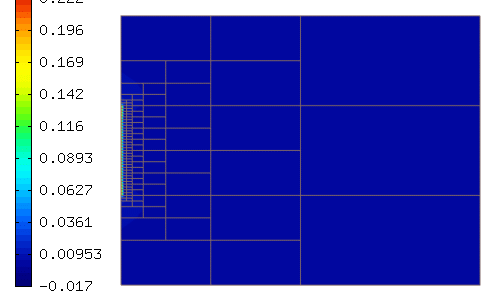
\includegraphics[width=0.33\textwidth]{img/acoustics/Solution_1.png}\hspace{1mm}
		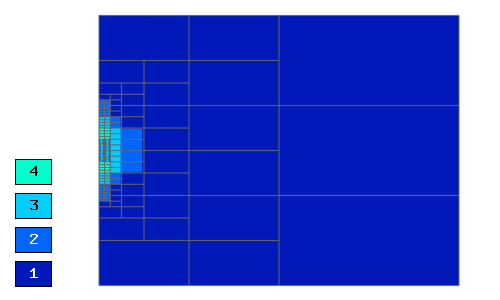
\includegraphics[width=0.33\textwidth]{img/acoustics/Space_1.png}\hspace{1mm}
		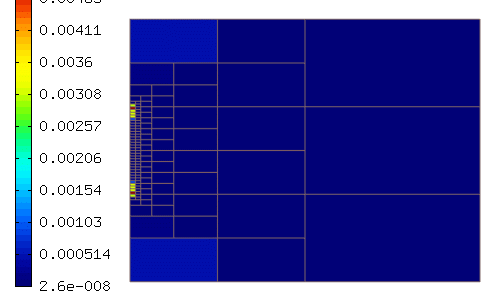
\includegraphics[width=0.33\textwidth]{img/acoustics/ErrorValue_1.png}\\
		\caption{Coarse solution, coarse space, and error in $p$; iteration = 1}
\vspace{5mm}
		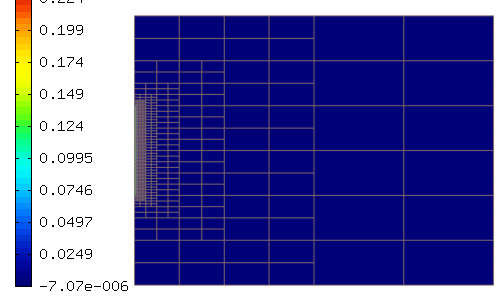
\includegraphics[width=0.33\textwidth]{img/acoustics/RefSolution_1.png}\hspace{1mm}
		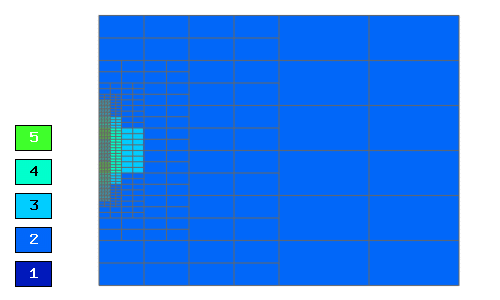
\includegraphics[width=0.33\textwidth]{img/acoustics/RefSpace_1.png}\hspace{1mm}
		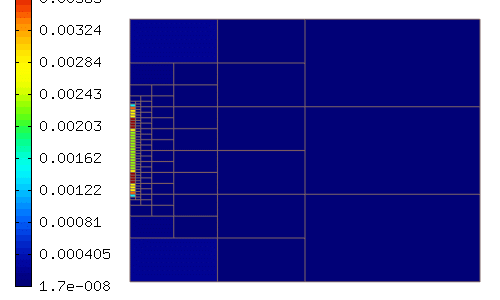
\includegraphics[width=0.33\textwidth]{img/acoustics/ErrorDerivative_1.png}\\
		\caption{Fine solution, fine space, and error in $\frac{\partial p}{\partial t}$; iteration = 1}
	\end{figure}

\textbf{Time step 45}
\begin{figure}[H]
		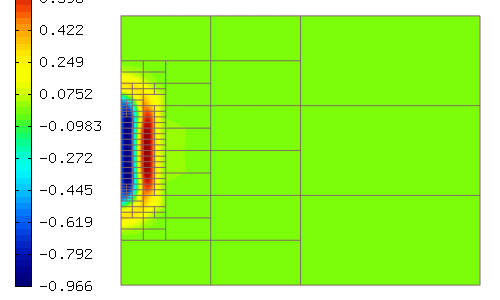
\includegraphics[width=0.33\textwidth]{img/acoustics/Solution_45.png}\hspace{1mm}
		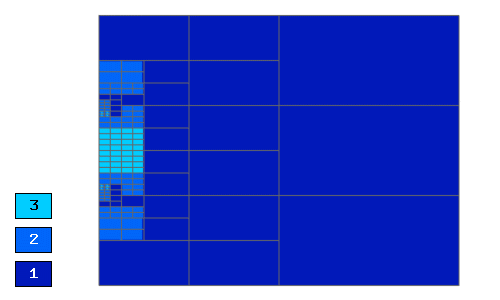
\includegraphics[width=0.33\textwidth]{img/acoustics/Space_45.png}\hspace{1mm}
		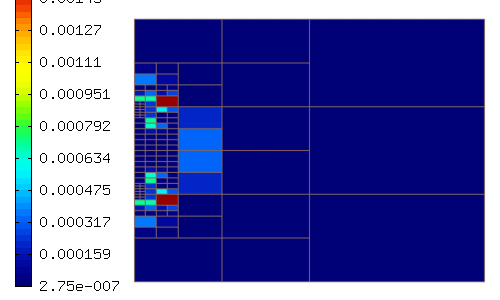
\includegraphics[width=0.33\textwidth]{img/acoustics/ErrorValue_45.png}\\
		\caption{Coarse solution, coarse space, and error in $p$; iteration = 45}
\vspace{5mm}
		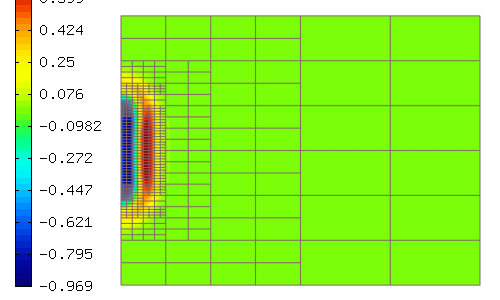
\includegraphics[width=0.33\textwidth]{img/acoustics/RefSolution_45.png}\hspace{1mm}
		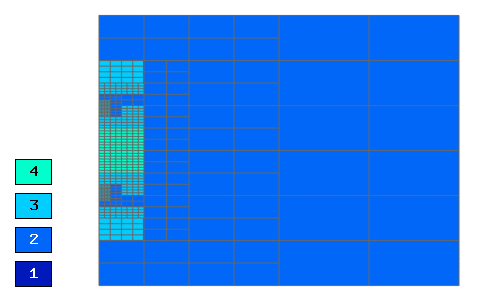
\includegraphics[width=0.33\textwidth]{img/acoustics/RefSpace_45.png}\hspace{1mm}
		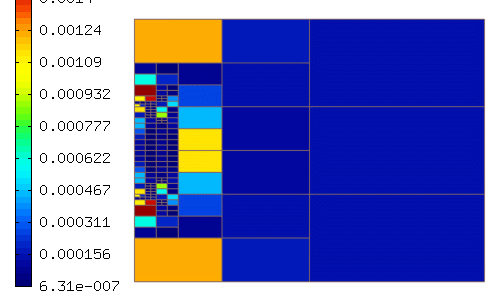
\includegraphics[width=0.33\textwidth]{img/acoustics/ErrorDerivative_45.png}\\
		\caption{Fine solution, fine space, and error in $\frac{\partial p}{\partial t}$; iteration = 45}
	\end{figure}
	
\textbf{Time step 90}
\begin{figure}[H]
		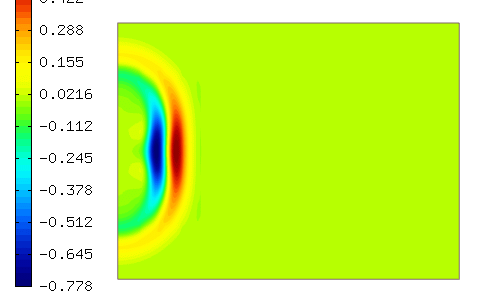
\includegraphics[width=0.33\textwidth]{img/acoustics/Solution_90.png}\hspace{1mm}
		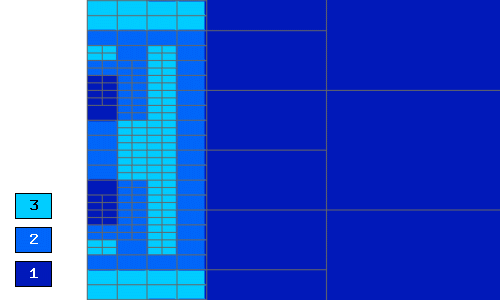
\includegraphics[width=0.33\textwidth]{img/acoustics/Space_90.png}\hspace{1mm}
		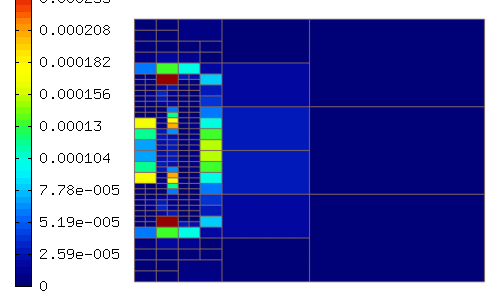
\includegraphics[width=0.33\textwidth]{img/acoustics/ErrorValue_90.png}\\
		\caption{Coarse solution, coarse space, and error in $p$; iteration = 90}
\vspace{5mm}
		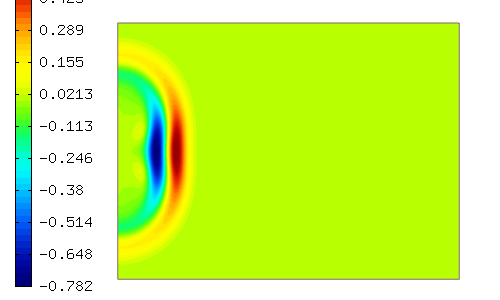
\includegraphics[width=0.33\textwidth]{img/acoustics/RefSolution_90.png}\hspace{1mm}
		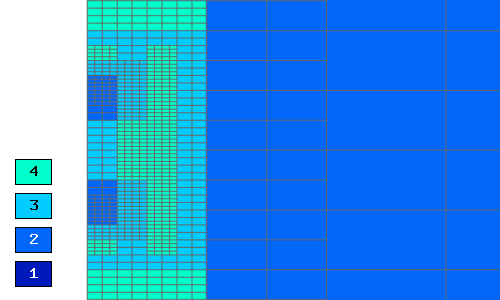
\includegraphics[width=0.33\textwidth]{img/acoustics/RefSpace_90.png}\hspace{1mm}
		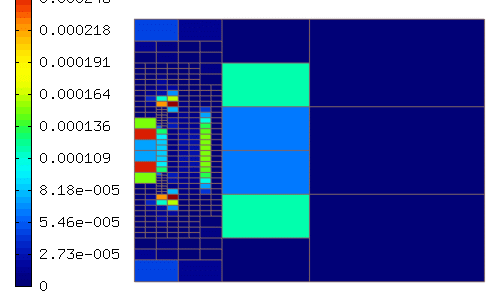
\includegraphics[width=0.33\textwidth]{img/acoustics/ErrorDerivative_90.png}\\
		\caption{Fine solution, fine space, and error in $\frac{\partial p}{\partial t}$; iteration = 90}
	\end{figure}
	
\textbf{Time step 134}
\begin{figure}[H]
		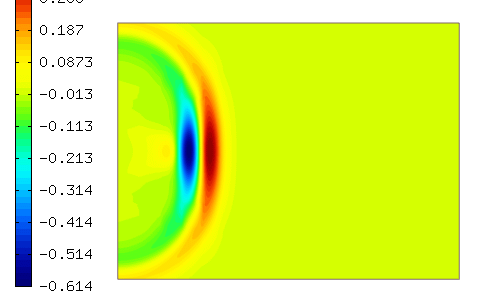
\includegraphics[width=0.33\textwidth]{img/acoustics/Solution_134.png}\hspace{1mm}
		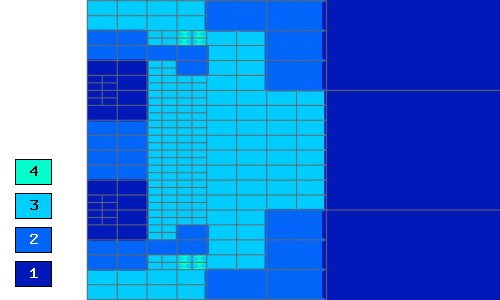
\includegraphics[width=0.33\textwidth]{img/acoustics/Space_134.png}\hspace{1mm}
		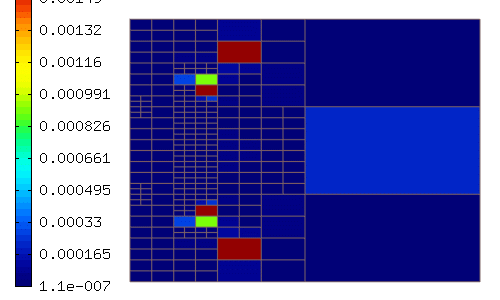
\includegraphics[width=0.33\textwidth]{img/acoustics/ErrorValue_134.png}\\
		\caption{Coarse solution, coarse space, and error in $p$; iteration = 134}
\vspace{5mm}
		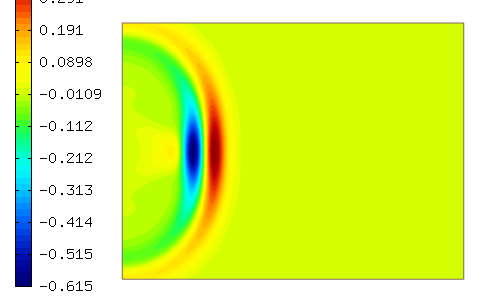
\includegraphics[width=0.33\textwidth]{img/acoustics/RefSolution_134.png}\hspace{1mm}
		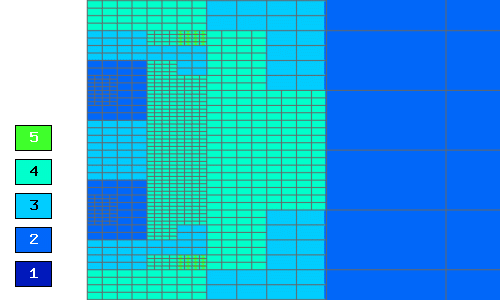
\includegraphics[width=0.33\textwidth]{img/acoustics/RefSpace_134.png}\hspace{1mm}
		\includegraphics[width=0.33\textwidth]{img/acoustics/ErrorDerivative_134.png}\\
		\caption{Fine solution, fine space, and error in $\frac{\partial p}{\partial t}$; iteration = 134}
	\end{figure}

\textbf{Time step 179}
\begin{figure}[H]
		\includegraphics[width=0.33\textwidth]{img/acoustics/Solution_179.png}\hspace{1mm}
		\includegraphics[width=0.33\textwidth]{img/acoustics/Space_179.png}\hspace{1mm}
		\includegraphics[width=0.33\textwidth]{img/acoustics/ErrorValue_179.png}\\
		\caption{Coarse solution, coarse space, and error in $p$; iteration = 179}
\vspace{5mm}
		\includegraphics[width=0.33\textwidth]{img/acoustics/RefSolution_179.png}\hspace{1mm}
		\includegraphics[width=0.33\textwidth]{img/acoustics/RefSpace_179.png}\hspace{1mm}
		\includegraphics[width=0.33\textwidth]{img/acoustics/ErrorDerivative_179.png}\\
		\caption{Fine solution, fine space, and error in $\frac{\partial p}{\partial t}$; iteration = 179}
	\end{figure}